\documentclass[12pt,a4paper]{article}
%\documentclass{aastex62}
\usepackage{aas_macros}
\usepackage{graphicx,amsmath,amssymb,float,subcaption,multirow,booktabs}
\usepackage[a4paper,top=15mm,bottom=15mm,left=35mm,right=15mm,marginparwidth=1.75cm]{geometry}
\usepackage[sort]{natbib}
\usepackage[toc,page]{appendix}
\usepackage[table,x11names]{xcolor}
\renewcommand{\baselinestretch}{1.5}

\bibliographystyle{humannat}
\title{Thesis}
\author{Andrew Nicholas Curzons}


\begin{document}


\pagebreak 

\newpage
\section{RX J1713.7-3946}

RX J1713.7-3946 is a galactic SNR first observed by the ROSAT all-sky survey at X-ray wavelengths \citep{1996rftu.proc..267P}. It is now one of the most extensively studied SNR's with strong TeV $\gamma$-ray emission as seen by HESS \citep{2004Natur.432...75A}. The precise particle origin of the $\gamma$-rays seen at the location of RX J1713.7-3946 is still unclear and remains the biggest question. Evidence for both a hadronic and leptonic model has been shown but the exact fraction of each is still unknown. We discuss such literature below.

\cite{1996rftu.proc..267P} derived a distance of 1.1 kpc and an age of 2100 years, with \cite{1997A&A...318L..59W} supported their claim following associations with the ancient Chinese quest star AD393.

After an initial detection by the ROSAT all-sky survey at energies between 0.1-2.4 keV, follow up observations with the Advanced Satellite for Cosmology and Astrophysics (ASCA) up to energies of 10 keV were made of the north-west region of the SNR \citep{1997PASJ...49L...7K}. X-rays of a thermal nature were ruled out due to the lack of line emission. A single power law was fitted to their data leading them to suspect that synchrotron processes were responsible for the emission, although at this point in time, no radio counterpart had been observed. The presence of synchrotron emission implies the presence of high energy electrons and subsequently that IC scattering should be occurring too. Thus, highlighting the importance of $\gamma$-ray observations in understanding cosmic ray acceleration. 

\cite{1999ApJ...525..357S} report no thermal X-ray emission from RX J1713.7-3946 and adopt a distance to the source of 6 kpc due to the likely association of the SNR with molecular clouds. They estimate the hydrogen density to be, $n_H = 0.034-0.69 d^{-1/2}$ cm$^{-3}$, where d is the distance to the source.

\cite{2000A&A...354L..57M} obtained the first TeV observations of RX J1713.7-3946 using the CANGAROO telescope. Their results showed that an extended region of $\gamma$-rays coincides with the spatial position of the X-rays. Further supporting the hypothesis that the high energy particles responsible for the emission are accelerated in shocks. Additionally, a pion decay model was ruled out due to it not reproducing the observed flux. The authors adopted a source distance and ISM gas density of 6 kpc and 0.28 cm$^{-3}$ respectively, from \cite{1999ApJ...525..357S}. For this reason they attributed the $\gamma$-ray flux to electrons undergoing IC scattering. However, the parameters used are not in agreement with other authors; \cite{1996rftu.proc..267P} derived a distance of 1.1 kpc and \cite{1997A&A...318L..59W} supported their claim following associations with the ancient Chinese quest star AD393.

\cite{2001ApJ...563..191E} present a nonlinear diffuse shock acceleration model in their broadband study of RX J1713.7-3946, using an electron population. Broadband fitting to the ASCA, CANGAROO and ATCA data enabled them to obtain realistic parameters for the magnetic field, explosion energy, matter density and other physical phenomena, most notably, $n_H$ approx. 0.01 cm$^{-3}$

\cite{2003A&A...400..567U} use the \textit{Chandra} X-ray observatory to reveal remarkably fine structure within the north-west rim of RX J1713.7-3946. Bright X-ray filaments are seen surrounded by fainter plateaus as well as a large circular void, which appears quite dim. Despite these variations in brightness, the spectral shape of the X-ray spectrum does not vary across the region. A synchrotron model was fitted to the X-ray data comfortably, however, the corresponding IC model could not explain the CANGAROO TeV observations. 

\cite{2003PASJ...55L..61F} looked towards CO gas located around the source for evidence of a hadronic scenario via the pion decay channel. They found a spatial correlation between a CO peak and the TeV $\gamma$-ray distribution, as measured by the CANGAROO experiment, concluding that CR protons ejected from the SNR must have interacted with this gas. They also showed that the CO distribution contains a hole which coincides with the X-ray emission seen by ROSAT. The identification of this gas at a velocity range from -11 to -3 km s$^{-1}$ also indicated that a distance of $\sim$ 1 kpc should be adopted for the SNR source.

\cite{2004ApJ...602..271L} compare X-ray and radio data from the \textit{Chandra X-ray Observatory} and ATCA, respectively. The morphology from both energy bands show some correlation, suggesting they originate from the same population of electrons. The differences in morphology are attributed to the difference in lifetime of electrons radiating at both energies (the radio-radiating electrons live up to 30 000 times longer), among other factors. No evidence of thermal X-ray emission was found. Steeper photon indices were found in fainter regions, suggesting that electrons are accelerated to higher energies in bright regions likely due to more intense magnetic fields. The broadband emission up to TeV energies is modeled with the synchrotron and IC scenarios. An average magnetic field strength less than 1 $\mu$G is needed to fit the models, allowing the fields to reach $\sim$15 $\mu$G in small regions. The maximum energy of electrons was deduced to be $\sim$5 TeV. 

\cite{2005A&A...431..953H} examine X-ray data from \textit{XMM-Newton} revealing more complex features and also a difference in spectra between the interior and western exterior of RX J1713.7-3946. They attribute this difference to either thermal X-rays originating in the central region or an increased column density in the western rim. The lack of thermal lines observed make the former hypothesis hard to justify. 

\cite{2005ApJ...631..947M} perform a detailed study of the molecular gas towards RX J1713.7-3946. They find a good correlation between the X-ray and gas distributions at velocities of -12 to -3 km s$^{-1}$, corresponding to a distance of 1 kpc for the SNR. They also show that the cloud previously thought to be interacting with the SNR at 6 kpc \citep{1999ApJ...525..357S} is not actually delineating the SNR boundary very well. Most of the CO peaks at 1 kpc are located just outside the SNR boundary, consistent with the shock front interacting with the gas from the inside out. The authors also find evidence of highly excited gas and broad wings in a particular gas peak, this is attributed to either shock interactions or effects from young stars. Finally they demonstrate how soft X-rays suffer from absorption by foreground gas. 

\cite{2004Natur.432...75A} obtain a higher resolution image of RX J1713.7-3946 using HESS. 
\cite{2006A&A...449..223A} confirmed 2003 measurements with much more significance (in the energy range 0.3-40 TeV). The $\gamma$-rays resemble a shell like structure, with brightest emission in the north-west and west and a void in the centre. Striking spatial correlation between $\gamma$-rays and X-rays observed by ASCA. Broadband model with parameters T = 1000 years, $n_H$ = 1 cm$^{-3}$ and D = 1kpc. IC peak was too narrow to reproduce the flat TeV emission. Bremsstrahlung only relevant for larger values of gas density, $n_H$ > 100 cm$^{-3}$. Models for the Hadronic scenario produced spectral shapes that are consistent with CR acceleration theory (10$^{51}$ erg energy budget of a SN). However the ISM gas density was not well constrained at this point in time. 
\cite{2007A&A...464..235A} find consistent results with the previous two studies using more HESS data. Their conclusions are the same as 2006, however they additionally show that protons and electrons are accelerated up to energies of 200 TeV and 100 TeV respectively in the region of RX J1713.7-3946. These energies are starting to approach the "knee". 

\cite{2007Natur.449..576U} discovered evidence of time variability of some of the X-ray hot spots/filaments, indicating that the magnetic field intensity should go beyond the order of a mG. This doesn't however refute leptonic models that require a much lower magnetic field strength ($\sim \mu$G) if they focus on regions larger than the filaments. The intense mG magnetic fields will average out with the extensive $\mu$G interstellar magnetic fields.


\cite{2008ApJ...685..988T} performed a morphological study and a spectral analysis to investigate the particle nature of the $\gamma$-rays. Firstly, their hadronic model contained a leptonic component to account for the X-ray and radio observations. While it fitted the spectral data well it also required a large magnetic field ($B = 200 \ \mu$G) and a small electron to proton ratio ($K_{ep} < 10^{-4}$). The leptonic model failed to account for the observed $\gamma$-ray flux at low TeV energies unless an extreme optical radiation density ($U_{rad} = 140$ ev cm$^{-3}$) was assumed for the IC process. Alternatively, they could have assumed an older age for the SNR ($>10^4$ years) to lower the energy break (equation \ref{eq:energybreak}) or included a separate electron population. Secondly, \cite{2008ApJ...685..988T} performed a morphological study between \textit{Suzaku} X-ray observations and HESS $\gamma$-ray observations. They found clear evidence of a spatial correlation between the two wavelengths. To account for this correlation and the success of the hadronic spectral model they attribute the X-ray emission to Synchrotron radiation and the $\gamma$-ray emission to PP interactions. They claim that the $\gamma$-ray radiation we see now is being produced over the entire life of the SNR remnant, whereas the X-ray radiation is due to a recent increase in injected electrons.

\cite{2009A&A...505..157A} make spatial and spectral comparisons between the X-rays and $\gamma$-rays towards RX J1713.7-3946. A non-linear correlation between the fluxes at both energies is found, $F_X \propto F_{\gamma}^{2.41}$. They argue that if the variation in flux is caused by variations in gas density then a leptonic model is preferred. Other results also lead them to favour a leptonic model over a hadronic model. The radial extent of the X-ray emission is shown to be smaller than that of the $\gamma$-ray emission. Lastly, they find evidence of a thermal origin for a bright radio arc and place it $\sim6.7$ kpc away, implying that it isn't connected to the SNR. 

\cite{2010ApJ...712..287E} argued that the amount of thermal X-ray line emission from RX J1713.7-3946 could be used to determine whether the IC scattering or PP scenario is more plausible. The hadronic PP model requires a certain target gas density and the thermal X-ray line emission scales as the gas density squared. So if the hadronic model requires a large proton density then this is incompatible with the lack of thermal X-rays from the source. A density of $n_H = 0.2$ cm$^{-3}$ was required for the hadronic model to meet the HESS observations. This resulted in a thermal X-ray model that greatly over-predicted the \textit{Suzaku} X-ray observations. At the same time a leptonic model was fitted to the HESS data with $n_H = 0.05$ cm$^{-3}$, this produced a thermal X-ray model that was compatible with the X-ray observations. For this reason \cite{2010ApJ...712..287E} favoured the leptonic model and ruled out the hadronic model.

\cite{2010ApJ...724...59S} make new observations of the dense cloud cores in the $^{12}$CO(J = 2-1) and $^{13}$CO(J = 2-1) transitions. They provide simulations that show that dense gas clumps can survive shock erosion due to the shock being stalled in the clumps. The dense cloud cores are rim-brightened in synchrotron emission where the magnetic field is enhanced. This indicates that the cores are located on the boundary of or within the SNR shell, e.g. they are physically associated with the X-rays. They attribute the broad wings seen at peak C \citep{2003PASJ...55L..61F, 2005ApJ...631..947M} to a protostar and not the SNR blast wave as previously considered. 

\cite{2011ApJ...735..120Y} performed a Monte Carlo simulation to separately explore the parameter space of a leptonic, hadronic and hybrid model in order to explain the multi-wavelength spectrum of RX J1713.7-3946. The hadronic model still contained a small leptonic contribution but the proton injection energy was dominant. The hybrid model required a larger contribution of the injection energy to electrons. The hybrid model also considered the scenario where the cut-off energy and spectral index for both the electron and proton distributions were equal. This resulted in the leptonic model having the smallest parameter space while the hadronic model required the largest. The goodness of fit was worst for the leptonic scenario and best for the hadronic scenario. An unrealistic injection energy was required for both the hadronic and hybrid models ($W_p > 4 \times 10^{51}$). On the other hand, the small parameter space of the leptonic model was more physically acceptable. Their work was inconclusive in regards to determining the nature of the parent particles.

\cite{2011ApJ...734...28A} presented observations of RX J1713.7-3946 by Fermi-LAT at $\gamma$-ray energies below that of HESS. They detect an extended source similar to that seen in X-rays and at higher $\gamma$-ray energies. A hard power law with a spectral index of 1.5 $\pm$ 0.1 is required to explain their observations between 500 MeV and 400 GeV. This finding is consistent with leptonic models of the $\gamma$-ray emission but not with hadronic models, leading the authors to favour IC scattering as the mechanism behind the $\gamma$-ray emission. They argued that there should still be some protons accelerated at the SNR, however, the target gas density is too low to invoke pion-decay interactions.

\cite{2012ApJ...751...65F} attempted to fit two purely leptonic models, both including radiative and adiabatic losses, to the RX J1713.7-3946 multi-wavelength spectrum. The first of which was a single zone model; the Synchrotron and IC emission originated from a single source. This model could not be perfectly fitted to the multi-wavelength spectral data. Their next model, a multi-zone model, included emission from compact knots, or regions of lower magnetic field strength. This provided a better fit to the observations emphasizing the need for fine scale variation in the magnetic field. 

\cite{2012ApJ...744...71I} study the effects of shocks interacting with gas clouds by performing 3D magnetohydrodynamical simulations. The magnetic field intensity can reach values of 1 mG at these interaction sites causing time variability of the synchrotron X-ray brightness, as observed by \cite{2007Natur.449..576U}. It also means that X-ray emission should correlate with the CO distribution on broad spatial scales. It is noted that the CO molecules may have been dissociated by the progenitor stars stellar wind and hence may not be observed. On much smaller scales the X-ray emission should show anti-correlation with the CO peaks, this is because the magnetic field amplification more strongly occurs at the boundary between the clouds and the diffuse gas. They further demonstrate how gas clumps with density $\gtrsim 10^3$ cm$^{-3}$ will survive the stellar wind and not be swept up (eq. \ref{eq:gas_dens_surv_shock}), leaving a diffuse inter-clump gas density of $\sim$0.01 cm$^{-3}$ within the SNR bubble.
\begin{equation} \label{eq:gas_dens_surv_shock}
n_H \gtrsim 10^3  \bigg( \dfrac{L_W}{10^{36} \text{ erg s}^{-1}} \bigg) \bigg( \dfrac{R_W}{10 \text{ pc}} \bigg)^{-5}  \bigg( \dfrac{t}{1000 \text{ yrs}} \bigg)^3 \text{ cm}^{-3}
\end{equation}
However, thermal X-rays are not expected to be emitted from the dense clumps, in accordance with observations (cite many studies), due to the decreased shock velocity at the shock-cloud interaction site causing the temperature to be suppressed locally. Lastly, they also show that the penetration depth of protons into dense clouds is energy dependent, hence they derive a hadronic $\gamma$-ray spectrum of 1.5, which is able to explain the $\gamma$-ray emission \citep{2011ApJ...734...28A}. The steepness of this spectrum is equivalent to that expected of the leptonic $\gamma$-rays, making the differentiation of the two processes difficult using spectral analysis alone. 

\cite{2012ApJ...746...82F} find such evidence in their study on the molecular and atomic gas towards RX J1713.7-3946. They combine data from the Nanten survey and the SGPS to obtain a total ISM proton density around the source ($n_H = 130$ cm$^{-3}$). The gas is shown to be shell like in nature, much like the $\gamma$-ray shell, with a cavity surrounded by dense clumps . This disreputes the idea that the hadronic model should be disregarded based on the work by \cite{2018arXiv180410579C}. \cite{2012ApJ...746...82F} also reveal a radial correlation between the gas and the $\gamma$-rays seen by HESS within the $\gamma$-ray shell. The evacuated cavity is interpreted as being formed by the stellar wind of the progenitor star. The velocity of the gas is also shown to be much less than the shock velocity, meaning that the shell distribution of gas we now observe is untouched by the shock front. The shell of $\gamma$-rays were predicted to have been produced in the last 100 or so years, based on their radial morphology and the speed of the shock, if indeed they are hadronic in nature. By calculating the penetration depths of both electrons and protons into the dense clouds, \cite{2012ApJ...746...82F} suggested how the protons would penetrate into the dense clumps producing $\gamma$-rays within, whereas the electrons would not penetrate the clumps and would remain at the acceleration site. This explains the spatial relationship between the target gas and the $\gamma$-rays and also proposes a method for the hadronic production of the $\gamma$-rays.

\cite{2013ApJ...778...59S} compare X-rays with 18 CO and HI clumps to find that the X-rays are enhanced around the clumps on a pc scale, while they are reduced inside the clumps on a 0.1 pc scale. The amplified magnetic field around the clumps enhances these synchrotron X-rays. The X-rays are weaker within the clumps due to the electrons not being able to penetrate the dense gas. The amplified magnetic field does not support a leptonic model. The clumps that are completely engulfed by the SNR are also completely surround by enhanced X-rays, while the clumps on the boundary of the SNR only have enhanced X-rays on their inside edge. Additionally, they find that X-ray absorption is negligible. 

Using CS(1-0) transitions, \cite{2013PASA...30...55M} identify new dense gas components towards Cores G and L, however it is unlikley that they're significantly contributing to the $\gamma$-ray emission due to their small mass. They find that a CR enhancement factor of 1000 fits with their model (Aharonian and Atoyan 1996). They also hypothesis a 'dark' component of gas, which is not detected by typical gas-tracers, arguing that it could make up above 30\% of the mass of observed gas clouds around RX J1713.7-3946. 

\cite{2014MNRAS.445L..70G} use a dynamical model to show that the hadronic scenario can explain the $\gamma$-ray emission if gas clumps are present. They assume that the SNR is transitioning between the ejacta-dominated and Sedov phase. A consequence of their model is the amplification of the magnetic field around the clumps. The magnetic field reaches intensities $\gtrsim 100 \mu$G at the clump boundaries and is as small as $\sim 10 \mu$G in the diffuse gas. The IC model is deemed negligible due to the high magnetic fields. Secondary electrons are also ignored due to their fast escape time from the clumps compared to their synchrotron and Bremsstrahlung cooling times. They describe how the CRs in their model make up $\sim$6\% of the total explosion energy and how this number should increase as the SNR ages. The absence of thermal X-rays agrees with their model. 

\cite{2015A&A...577A..12F} build on the work from \cite{2011ApJ...734...28A}, using more up to date Fermi-LAT data. They measure a hard spectrum, $\alpha = 1.53 \pm 0.07$, as measured with earlier LAT data. The hard spectrum is shown to be compatible with a hadronic model if a CR precursor to the forward shock is considered. The hadronic $\gamma$-ray emission is shown to increase by $\sim$15\% over a 10 year period as a result of this model. This variation should be detectable with the CTA. 

\cite{2015ApJ...799..175S} use high resolution X-ray spectral data to compare the X-ray properties with interstellar gas in 305 regions around RX J1713.7-3946. The X-ray intensity is shown to be well correlated with the X-ray photon index in the western region of the SNR. They find that the photon index is distributed as "small islands" of lower values and is anti-correlated with the X-rays. They confirm the correlation of X-rays and gas on pc scales and the anti-correlation of X-rays and gas on sub-parsec scales as per previous work \citep{2010ApJ...724...59S, 2013ApJ...778...59S}. The ISM is rich in the western half of the region, suggesting that the shock-cloud interactions are more effective here. 


\cite{2015ApJ...814...29K} reported the first detection of thermal X-ray line emission using \textit{Suzaku} and \textit{XMM-Newton} observations. They attribute the emission to reverse-shocked SN ejecta as opposed to shocked ISM gas. Their study focused on the interior region, which contains softer X-rays, helpful as less absorption of the thermal X-rays occurs and the synchrotron emission is weaker. 


\cite{2016ApJ...821...43Z} use two different two-zone models to recreate the observed broadband spectrum, notably, the hard GeV $\gamma$-ray spectrum. Both of these models assume a hadronic component for the outer zone, e.g. diffusive protons that have escaped from the shock front interact with the surrounding gas clouds. The remaining zone, the inner zone, is modeled either as IC scattering or as proton interactions with shocked clumps. The main contribution to the GeV emission in both models is from the escaping protons interacting in the outer zone. Both models can also explain the radial profile of the TeV $\gamma$-rays seen by HESS that extends beyond that of the X-ray profile. They suggest that this outer emitting region in the TeV band is due to the escaping protons. The dominant component for the inner zone in each model is determined by the the electron to proton ratio, $K_{ep}$, being above or below $\sim 4 \times 10^3$. 

\cite{2017IAUS..331..206K} report on further thermal X-ray line emission, covering a larger region than \cite{2015ApJ...814...29K}, yet still analysing the softer interior. They additionally derive an upstream density to be $\sim$0.01 cm$^{-3}$, compatible with the shocked ISM not producing thermal X-rays. They suggest a core-collapse SN due to the Fe deficit and also estimate an age of $\sim$1200-1600 years.

\cite{2017JHEAp..13...17O} explain two results from \cite{2018A&A...612A...6H} with an IC model. These results are that there is a break in the $\gamma$-ray spectrum at 100 GeV and that the $\gamma$-ray spectrum is more extended than the X-ray spectrum. Their model showed the maximum energy of currently accelerated electrons is 5 TeV, which cannot emit X-rays above 0.1 keV or $\gamma$-rays above a few TeV. 

\cite{2017ApJ...840...74A} run simulations to highlight the potential capabilities of CTA with regards to observations of RX J1713.7-3946. They predict that the particle origin of the $\gamma$-ray emission will be identifiable using the high resolution morphology seen by CTA. They also claim that a possible hidden hadronic component may be detectable as well as time variations of the cut-off energy of the $\gamma$-ray spectrum. CTA will measure $\gamma$-rays with energies well below 0.3 TeV, in the hope of revealing a break in the spectrum at $\sim$0.3 TeV. Finally, they acknowledge the claims of thermal X-rays \citep{2015ApJ...814...29K} as negligible in regards to either a leptonic or hadronic model. 

\cite{2018arXiv180410579C} build on work from \cite{2012ApJ...744...71I,2014MNRAS.445L..70G} to show that a hadronic model should not be ruled out. They investigated how the SNR shock front interacts with inhomogeneities in molecular gas clouds and invoked a magneto-hydrodynamical model. The inhomogeneities are represented by regions of highly dense molecular clumps. The magnetic fields around potential dense clumps are intensified as the shock propagates around them. In such a case, low energy particles were shown to require more time to penetrate the clumps, due to the intensified magnetic field, in comparison to high energy particles. Subsequently, the energy spectrum at GeV energies becomes harder inside the clumps. This could be used to explain why the Fermi-LAT observations require a hard spectrum. The clumps also remain relatively un-shocked, i.e. their morphology isn't affected, and hence remain cold. This is argued to be the reason for the lack of thermal X-ray observations from RX J1713.7-3946. Gas studies cannot resolve gas clumps of the scale referred to in this study (0.1 pc) but they could be used to find evidence of larger clumps.


The latest work done by the HESS collaboration shows that both a pure leptonic and a pure hadronic model can be used to explain observations that have been made (\cite{2018A&A...612A...6H}, henceforth H16). This study also presented the latest observations by HESS, with a resolution that can be used to constrain, not only the remnant as a whole, but 29 smaller regions in TeV $\gamma$-rays (Figure \ref{fig:hesssubregions}).
\begin{figure}[H]
	\centering
	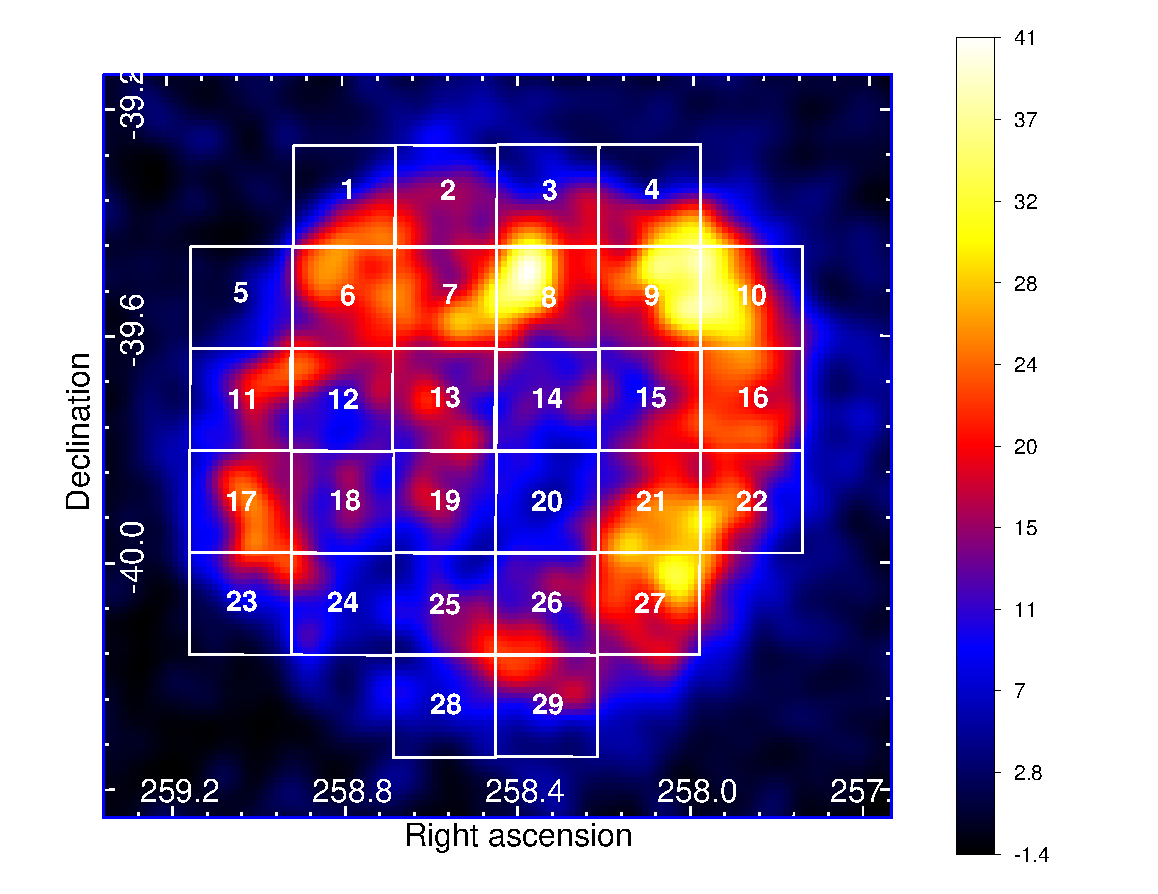
\includegraphics[width=0.7\linewidth, height=0.34\textheight]{HESS_subregions}
	\caption{HESS $\gamma$-ray image of RX J1713.7-3946 for energies greater than 2 TeV. The overlaid white squares represent the 29 sub regions.}
	\label{fig:hesssubregions}
\end{figure}
This data can be simultaneously used with \textit{Suzaku} X-ray observations, which have also been resolved to the same 29 regions \citep{2008ApJ...685..988T}, to constrain any models seeking to probe into the finer, small scale details of RX J1713.7-3946. HESS showed that these 29 sub regions can also be explained by either a pure leptonic or a pure hadronic model. Other constraints are imposed by Fermi-LAT observations at GeV-TeV $\gamma$-ray energies and ATCA radio observations \citep{2004ApJ...602..271L}. However, Fermi-LAT observations fail to resolve the fine detail needed to examine regional parts of the SNR.



The majority of studies discussed have failed to address the importance of Bremsstrahlung radiation, if any at all. One study included a Bremsstrahlung contribution in their leptonic model and found that the effects were minimal \citep{2012ApJ...751...65F} (how/why?). There are also no meaningful constraints at MeV energies where Bremsstrahlung can often be dominant, for these reasons it is often neglected.



\bibliography{bibliography}

\end{document}